\documentclass[11pt]{ctexart}

% set 1-inch margins in the document
\usepackage[margin=1in]{geometry}
\usepackage{amsthm}
\usepackage{tikz}
\usetikzlibrary{automata}

% include this if you want to import graphics files with /includegraphics
\usepackage{graphicx}

\author{宋赟祖}
\begin{document}
	\begin{enumerate}
		\item 关键字\\
		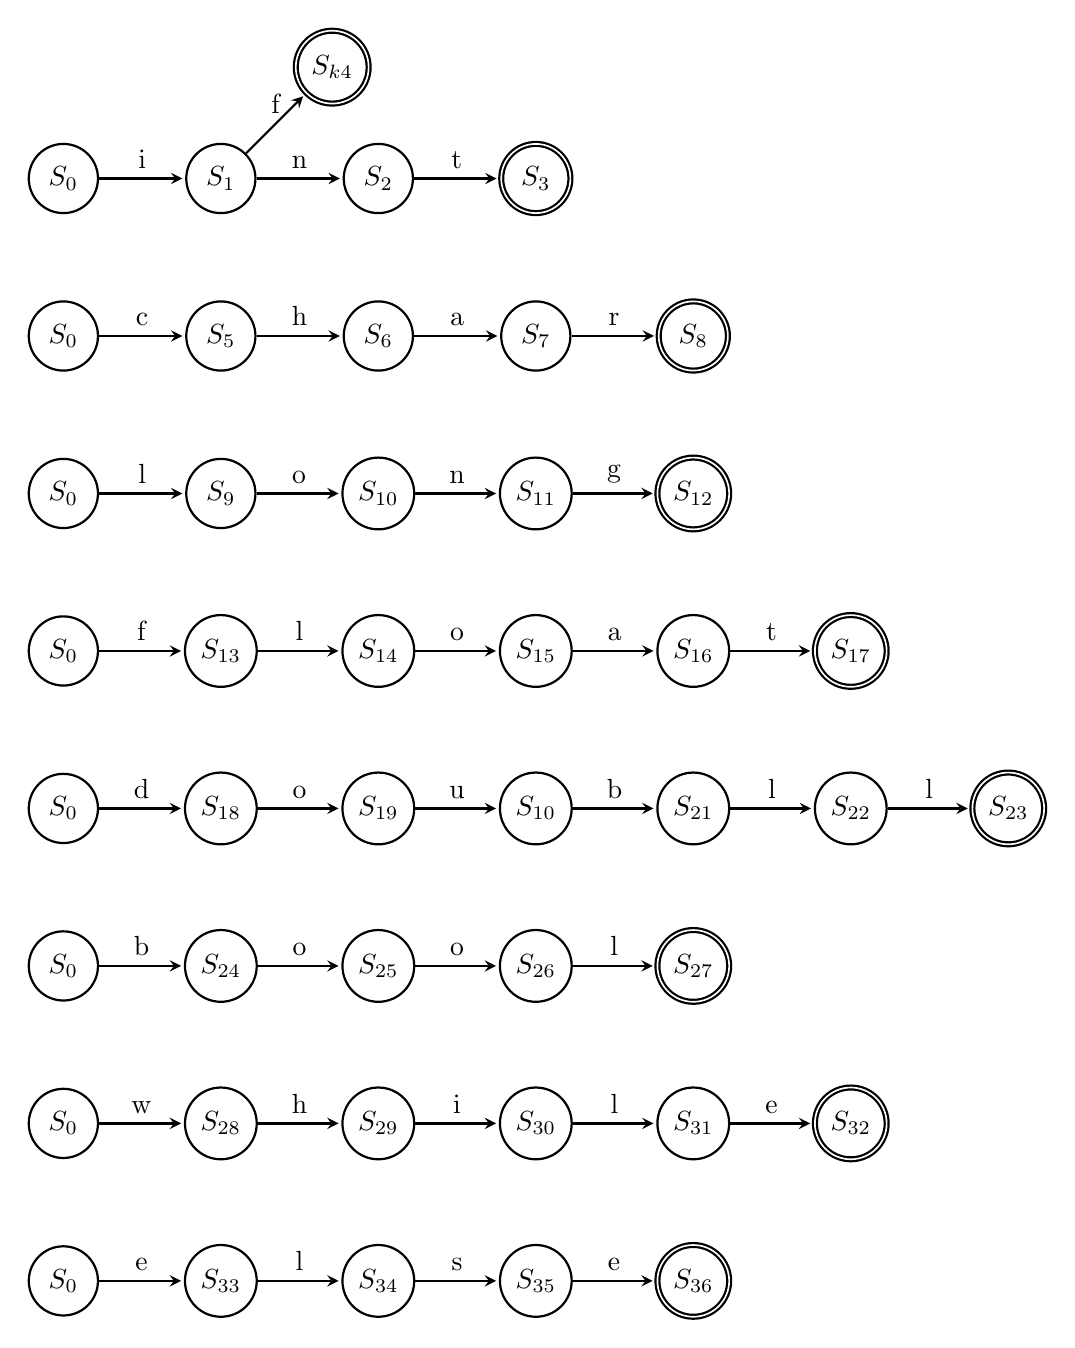
\begin{tikzpicture}[->,>=stealth,shorten >=1pt,auto,node distance=2cm,
		thick,base node/.style={circle,draw,minimum size=16pt}, real node/.style={double,circle,draw,minimum size=35pt}]
		
		% int if
		\node[state] (k1) {$S_{0}$};
		\node[state] (k2) [right of= k1]{$S_{1}$};
		\node[state] (k3) [right of= k2]{$S_{2}$};
		\node[state, accepting] (k4) [right of= k3]{$S_{3}$};
		\node[state, accepting] (k34) [above right of= k2]{$S_{k4}$};
		\path[->]
		(k1) edge node [above] {i} (k2)
		(k2) edge node [above] {n} (k3)
		(k3) edge node [above] {t} (k4)
		(k2) edge node [above] {f} (k34);
		
		% char
		\node[state] (k5) [below of=k1]{$S_{0}$};
		\node[state] (k6) [right of= k5]{$S_{5}$};
		\node[state] (k7) [right of= k6]{$S_{6}$};
		\node[state] (k8) [right of= k7]{$S_{7}$};
		\node[state, accepting] (k9) [right of= k8]{$S_{8}$};
		\path[->]
		(k5) edge node [above] {c} (k6)
		(k6) edge node [above] {h} (k7)
		(k7) edge node [above] {a} (k8)
		(k8) edge node [above] {r} (k9);
		
		% long
		\node[state] (k10) [below of=k5]{$S_{0}$};
		\node[state] (k11) [right of= k10]{$S_{9}$};
		\node[state] (k12) [right of= k11]{$S_{10}$};
		\node[state] (k13) [right of= k12]{$S_{11}$};
		\node[state, accepting] (k14) [right of= k13]{$S_{12}$};
		\path[->]
		(k10) edge node [above] {l} (k11)
		(k11) edge node [above] {o} (k12)
		(k12) edge node [above] {n} (k13)
		(k13) edge node [above] {g} (k14);
		
		% float
		\node[state] (k16) [below of=k10]{$S_{0}$};
		\node[state] (k17) [right of= k16]{$S_{13}$};
		\node[state] (k18) [right of= k17]{$S_{14}$};
		\node[state] (k19) [right of= k18]{$S_{15}$};
		\node[state] (k20) [right of= k19]{$S_{16}$};
		\node[state, accepting] (k21) [right of= k20]{$S_{17}$};
		\path[->]
		(k16) edge node [above] {f} (k17)
		(k17) edge node [above] {l} (k18)
		(k18) edge node [above] {o} (k19)
		(k19) edge node [above] {a} (k20)
		(k20) edge node [above] {t} (k21);
		
		% double do
		\node[state] (k22) [below of=k16]{$S_{0}$};
		\node[state] (k23) [right of= k22]{$S_{18}$};
		\node[state] (k24) [right of= k23]{$S_{19}$};
		\node[state] (k25) [right of= k24]{$S_{10}$};
		\node[state] (k26) [right of= k25]{$S_{21}$};
		\node[state] (k27) [right of= k26]{$S_{22}$};
		\node[state, accepting] (k28) [right of= k27]{$S_{23}$};
		\path[->]
		(k22) edge node [above] {d} (k23)
		(k23) edge node [above] {o} (k24)
		(k24) edge node [above] {u} (k25)
		(k25) edge node [above] {b} (k26)
		(k26) edge node [above] {l} (k27)
		(k27) edge node [above] {l} (k28);
		
		% bool
		\node[state] (k29) [below of=k22]{$S_{0}$};
		\node[state] (k30) [right of= k29]{$S_{24}$};
		\node[state] (k31) [right of= k30]{$S_{25}$};
		\node[state] (k32) [right of= k31]{$S_{26}$};
		\node[state, accepting] (k33) [right of= k32]{$S_{27}$};
		\path[->]
		(k29) edge node [above] {b} (k30)
		(k30) edge node [above] {o} (k31)
		(k31) edge node [above] {o} (k32)
		(k32) edge node [above] {l} (k33);
		
		
		% while
		\node[state] (k35) [below of=k29]{$S_{0}$};
		\node[state] (k36) [right of= k35]{$S_{28}$};
		\node[state] (k37) [right of= k36]{$S_{29}$};
		\node[state] (k38) [right of= k37]{$S_{30}$};
		\node[state] (k39) [right of= k38]{$S_{31}$};
		\node[state, accepting] (k40) [right of= k39]{$S_{32}$};
		\path[->]
		(k35) edge node [above] {w} (k36)
		(k36) edge node [above] {h} (k37)
		(k37) edge node [above] {i} (k38)
		(k38) edge node [above] {l} (k39)
		(k39) edge node [above] {e} (k40);
		
		% else
		\node[state] (k41) [below of=k35]{$S_{0}$};
		\node[state] (k42) [right of= k41]{$S_{33}$};
		\node[state] (k43) [right of= k42]{$S_{34}$};
		\node[state] (k44) [right of= k43]{$S_{35}$};
		\node[state, accepting] (k45) [right of= k44]{$S_{36}$};
		\path[->]
		(k41) edge node [above] {e} (k42)
		(k42) edge node [above] {l} (k43)
		(k43) edge node [above] {s} (k44)
		(k44) edge node [above] {e} (k45);
		\end{tikzpicture}
		
		\item 连接\\
		
		\begin{tikzpicture}[->,>=stealth,shorten >=1pt,auto,node distance=4cm,
		thick,base node/.style={circle,draw,minimum size=12pt}, real node/.style={double,circle,draw,minimum size=35pt}]
		% connection
		\node[state] (keys) [below of=k42]{$S_{1-36}$};
		\node[state] (goto) [right of= keys]{$S_{55}$};
		\path[->]
		(keys) edge node [above] {letter/digit} (goto);
		\end{tikzpicture}
		
		\item 算术运算符\\
		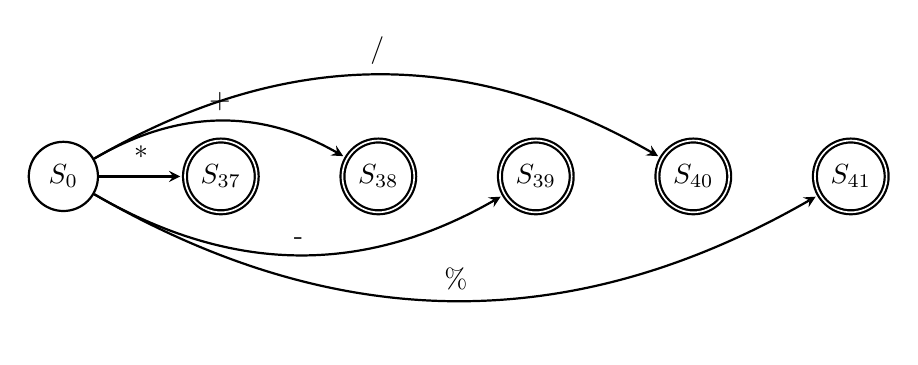
\begin{tikzpicture}[->,>=stealth,shorten >=1pt,auto,node distance=2cm,
		thick,base node/.style={circle,draw,minimum size=12pt}, real node/.style={double,circle,draw,minimum size=35pt}]
		% 算术运算符
		\node[state] (op1) {$S_{0}$};
		\node[state, accepting] (op2) [right of= op1]{$S_{37}$};
		\node[state, accepting] (op3) [right of= op2]{$S_{38}$};
		\node[state, accepting] (op4) [right of= op3]{$S_{39}$};
		\node[state, accepting] (op5) [right of= op4]{$S_{40}$};
		\node[state, accepting] (op6) [right of= op5]{$S_{41}$};
		\path[->]
		(op1) edge node [above] {*} (op2)
		(op1) edge [bend left] node  {+} (op3)
		(op1) edge [bend right] node  {-} (op4)
		(op1) edge [bend left] node  {/} (op5)
		(op1) edge [bend right] node  {\%} (op6);
		\end{tikzpicture}
		
		\item 逻辑运算符 关系运算符\\
		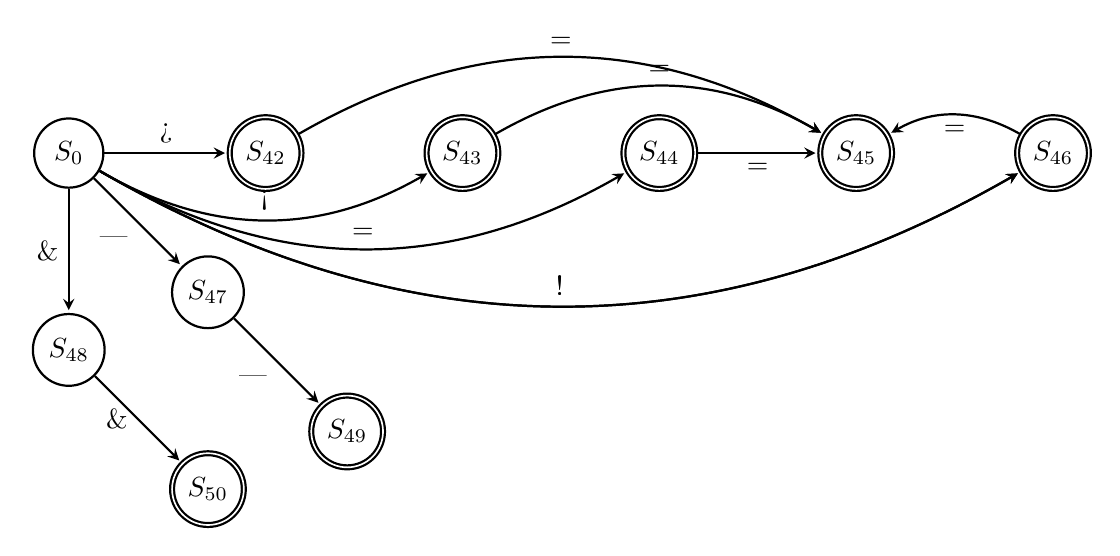
\begin{tikzpicture}[->,>=stealth,shorten >=1pt,auto,node distance=2.5cm,
		thick,base node/.style={circle,draw,minimum size=12pt}, real node/.style={double,circle,draw,minimum size=35pt}]
		% 逻辑运算符
		\node[state] (op7){$S_{0}$};
		\node[state, accepting] (op8) [right of= op7]{$S_{42}$};
		\node[state, accepting] (op9) [right of= op8]{$S_{43}$};
		\node[state, accepting] (op10) [right of= op9]{$S_{44}$};
		\node[state, accepting] (op11) [right of= op10]{$S_{45}$};
		\node[state, accepting] (op12) [right of= op11]{$S_{46}$};
		\node[state] (op13) [below right of= op7]{$S_{47}$};
		\node[state] (op14) [below of= op7]{$S_{48}$};
		\node[state, accepting] (op15) [below right of= op13]{$S_{49}$};
		\node[state, accepting] (op16) [below right of= op14]{$S_{50}$};
		\path[->]
		(op7) edge node [above] {>} (op8)
		(op7) edge [bend right] node  {<} (op9)
		(op7) edge [bend right] node  {=} (op10)
		(op10) edge [below] node  {=} (op11)
		(op7) edge [bend right] node  {!} (op12)
		(op12) edge [bend right] node  {=} (op11)
		(op8) edge [bend left] node  {=} (op11)
		(op9) edge [bend left] node  {=} (op11)
		(op7) edge [bend right] node  {!} (op12)
		(op7) edge [below left] node  {|} (op13)
		(op13) edge [below left] node  {|} (op15)
		(op7) edge [left] node  {\&} (op14)
		(op14) edge [left] node  {\&} (op16);
		\end{tikzpicture}
		
		\item 界符\\
		
		\begin{tikzpicture}[->,>=stealth,shorten >=1pt,auto,node distance=2.5cm,
		thick,base node/.style={circle,draw,minimum size=12pt}, real node/.style={double,circle,draw,minimum size=35pt}]
		% 界符
		\node[state] (b1) [below left of= op16]{$S_{0}$};
		\node[state, accepting] (b2) [right of= b1]{$S_{51}$};
		\node[state, accepting] (b3) [right of= b2]{$S_{52}$};
		\node[state, accepting] (b4) [right of= b3]{$S_{53}$};
		\node[state, accepting] (b5) [right of= b4]{$S_{54}$};
		\node[state, accepting] (b6) [above of= b1]{$S_{75}$};
		\node[state, accepting] (b7) [below of= b1]{$S_{76}$};
		
		\path[->]
		(b1) edge node [above] {;} (b2)
		(b1) edge [bend right] node  {[} (b3)
		(b1) edge [bend left] node  {]} (b4)
		(b1) edge [bend right] node  {.} (b5)
		(b1) edge [left] node  {\}} (b6)
		(b1) edge [left] node  {\{} (b7);
		\end{tikzpicture}
		
		\item 标识符\\
		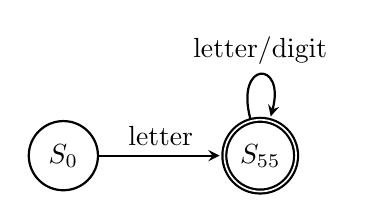
\begin{tikzpicture}[->,>=stealth,shorten >=1pt,auto,node distance=2.5cm,
		thick,base node/.style={circle,draw,minimum size=12pt}, real node/.style={double,circle,draw,minimum size=35pt}]
		% 标识符
		
		\node[state] (id1) {$S_{0}$};
		\node[state, accepting] (id2) [right of= id1]{$S_{55}$};
		\path[->]
		(id1) edge node [above] {letter} (id2)
		(id2) edge [loop above] node  {letter/digit} (id2);
		\end{tikzpicture}
		
		\item 常数\\
		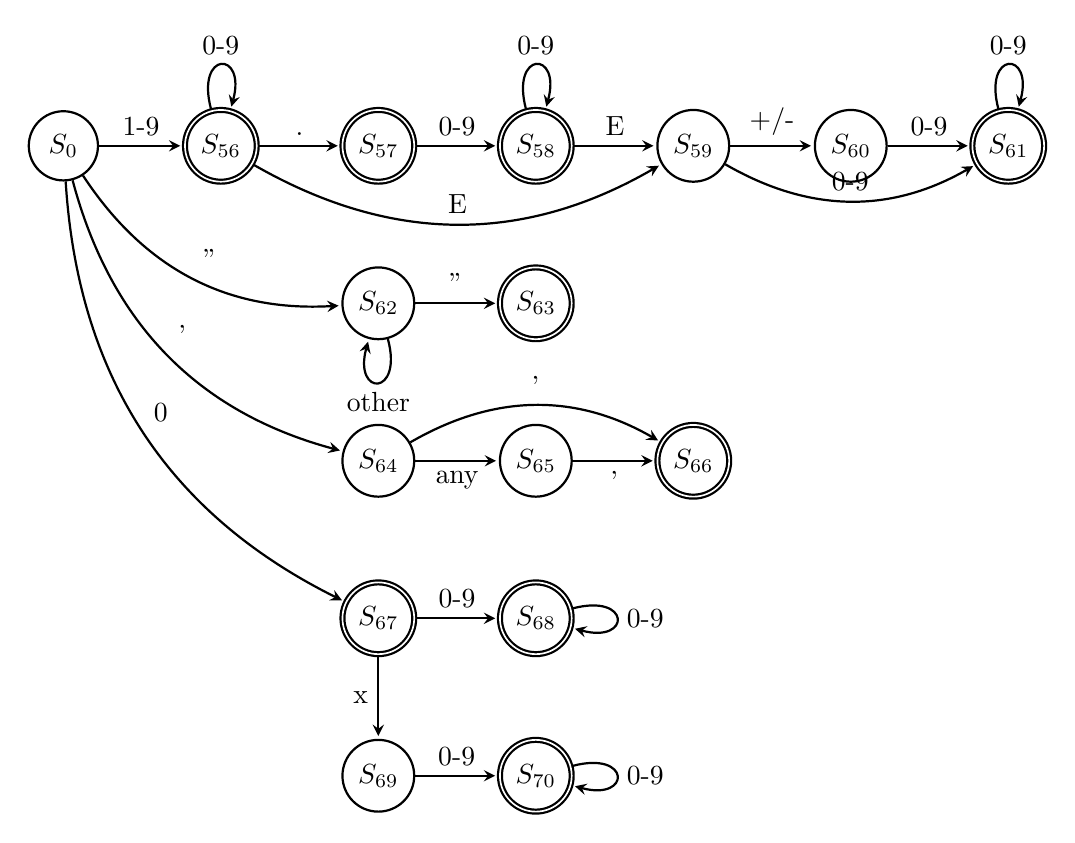
\begin{tikzpicture}[->,>=stealth,shorten >=1pt,auto,node distance=2cm,
		thick,base node/.style={circle,draw,minimum size=12pt}, real node/.style={double,circle,draw,minimum size=35pt}]
		% 常数
		\node[state] (c1) {$S_{0}$};
		\node[state, accepting] (c2) [right of= c1]{$S_{56}$};
		\node[state, accepting] (c3) [right of= c2]{$S_{57}$};
		\node[state, accepting] (c4) [right of= c3]{$S_{58}$};
		\node[state] (c5) [right of= c4]{$S_{59}$};
		\node[state] (c6) [right of= c5]{$S_{60}$};
		\node[state, accepting] (c7) [right of= c6]{$S_{61}$};
		% 字符串常数
		\node[state] (c8) [below of= c3]{$S_{62}$};
		\node[state, accepting] (c11) [right of= c8]{$S_{63}$};
		
		% 字符常数
		\node[state] (c9) [below of= c8]{$S_{64}$};
		\node[state] (c12) [right of= c9]{$S_{65}$};
		\node[state, accepting] (c13) [right of= c12]{$S_{66}$};
		
		% 八进制常数 十六进制常数
		\node[state, accepting] (c10) [below of= c9]{$S_{67}$};
		\node[state, accepting] (c14) [right of= c10]{$S_{68}$};
		\node[state] (c15) [below of= c10]{$S_{69}$};
		\node[state, accepting] (c16) [right of= c15]{$S_{70}$};
		
		\path[->]
		(c1) edge node [above] {1-9} (c2)
		(c2) edge [loop above] node  {0-9} (c2)
		(c2) edge [above] node  {.} (c3)
		(c3) edge [above] node  {0-9} (c4)
		(c4) edge [loop above] node  {0-9} (c4)
		(c4) edge [above] node  {E} (c5)
		(c2) edge [bend right] node  {E} (c5)
		(c5) edge [above] node  {+/-} (c6)
		(c5) edge [bend right] node  {0-9} (c7)
		(c6) edge [above] node  {0-9} (c7)
		(c7) edge [loop above] node  {0-9} (c7)
		
		% 字符串
		(c1) edge [bend right] node  {"} (c8)
		(c8) edge [loop below] node  {other} (c8)
		(c8) edge [above] node  {"} (c11)
		
		
		% 字符常数
		(c1) edge [bend right] node  {'} (c9)
		(c9) edge [below] node  {any} (c12)
		(c12) edge [below] node  {'} (c13)
		(c9) edge [bend left] node  {'} (c13)
		
		% 八进制
		(c1) edge [bend right] node  {0} (c10)
		(c10) edge [above] node  {0-9} (c14)
		(c10) edge [left] node  {x} (c15)
		(c14) edge [loop right] node  {0-9} (c14)
		(c15) edge [above] node  {0-9} (c16)
		(c16) edge [loop right] node  {0-9} (c16);
		
		\end{tikzpicture}
	
		
		\item 注释 \\
		% 注释
		\begin{tikzpicture}[->,>=stealth,shorten >=1pt,auto,node distance=2cm,
		thick,base node/.style={circle,draw,minimum size=12pt}, real node/.style={double,circle,draw,minimum size=35pt}]
		\node[state] (com1) {$S_{0}$};
		\node[state] (com2) [right of= com1]{$S_{71}$};
		\node[state] (com3) [right of= com2]{$S_{72}$};
		\node[state] (com4) [right of= com3]{$S_{73}$};
		\node[state, accepting] (com5) [right of= com4]{$S_{74}$};
		\path[->]
		(com1) edge node [above] {/} (com2)
		(com2) edge [above] node  {*} (com3)
		(com3) edge [loop above] node  {other} (com3)
		(com3) edge [above] node  {*} (com4)
		(com4) edge [bend left] node  {other} (com3)
		(com4) edge [loop above] node  {*} (com4)
		(com4) edge [above] node  {/} (c5);
		\end{tikzpicture}
		
		
	\end{enumerate}
	
	
	
	
	
	
	
	
	
	
	
	
\end{document}

